\documentclass[hidelinks,aspectratio=169]{beamer}
\usepackage[italian]{babel} 
\usepackage[utf8]{inputenc} 
\usepackage{fourier} 

%Slide colors
\usetheme{Madrid}
%\usecolortheme{beaver}

% Images
\usepackage{graphicx}
\usepackage{caption}
\usepackage{subcaption}
\usepackage{float}
\graphicspath{{Images}}

% Stop hyphenation
\usepackage[none]{hyphenat}

% Minipages in the same line
\usepackage{tabularx}

% Coloring links
\usepackage{xcolor}

% Enumerate abc
\usepackage{enumerate}

% Redefines caption setup in way to remove "Figure:"
\usepackage{caption}
\captionsetup[figure]{labelformat=empty}

% License
\usepackage[
type={CC},
modifier={by-nc-sa},
version={4.0},
]{doclicense}

%------------------- Commands zone --------------------

%Command to zoom in
\usepackage{mwe}
\makeatletter
\newsavebox\zb@x
\newcounter{z@@m}
\usepackage{calc}
\newdimen\B@r\newdimen\P@r
\newdimen\@zw\newdimen\@zh\newdimen\@zd

\newcommand{\zoombox}[2][0]{%
	\leavevmode%
	\sbox\zb@x{#2}%
	\setlength\B@r{1pt*\ratio{\wd\zb@x}{\ht\zb@x+\dp\zb@x}}%
	\setlength\P@r{1pt*\ratio{\paperwidth}{\paperheight}}%
	\ifdim\B@r>\P@r\relax%
	\setlength\@zw{\wd\zb@x}\setlength\@zh{\@zw*\ratio{\paperheight}{\paperwidth}}%
	\setlength\@zd{(\@zh-\ht\zb@x-\dp\zb@x)*\real{0.5}+\dp\zb@x}%
	\setlength\@zh{\@zh-\@zd}%
	\else%
	\setlength\@zh{\ht\zb@x+\dp\zb@x}%
	\setlength\@zw{\@zh*\ratio{\paperwidth}{\paperheight}}%
	\setlength\@zh{\ht\zb@x}\setlength\@zd{\dp\zb@x}%
	\fi%
	\makebox[0pt][l]{\makebox[\wd\zb@x][c]{\makebox[\@zw][l]{%
				\pdfdest name {zbfs\thez@@m} fitr
				width  \@zw\space
				height \@zh\space
				depth  \@zd\space
	}}}%
	\pdfdest name {zb\thez@@m} fitr
	width  \wd\zb@x\space
	height \ht\zb@x\space
	depth  \dp\zb@x\space
	\immediate\pdfannot 
	width  \wd\zb@x\space
	height \ht\zb@x\space
	depth  \dp\zb@x\space
	{%
		/Subtype/Link/H/N
		/Border [0 0 #1 [1 2]]
		/A <<
		/S/JavaScript
		/JS (
		if(typeof(zoomed)=='undefined'||!zoomed){
			var lastView=this.viewState;
			if(app.fs.isFullScreen) this.gotoNamedDest('zbfs\thez@@m');
			else this.gotoNamedDest('zb\thez@@m');
			zoomed=true;
		}else{
			this.viewState=lastView;
			zoomed=false;
		}
		)
		>>
	}%
	\usebox{\zb@x}%
	\stepcounter{z@@m}%
} 
\makeatother

%------------------- Header --------------------
\title[Dispositivo anti-collega rumoroso IoT]{\small \textbf{Dispositivo anti-collega rumoroso IoT}}
\author[Francesco Rombaldoni]{}
\date{Anno Accademico 2025/2026}

\begin{document}
	
	\begin{frame}
		\vspace*{-5mm}
		\begin{center}
			\hspace*{30mm}\zoombox{
\includegraphics[scale=0.2]{logo-uniurb-2016.jpg}}
			\vspace*{2mm}
			\newline
			{\Large UNIVERSITÀ DEGLI STUDI DI URBINO CARLO BO}\\
			\vspace*{0.5mm}
			Dipartimento di Scienze Pure e Applicate\\
			\vspace*{0.5mm}
			Corso di Laurea in informatica e innovazione digitale\\
			%\vspace*{0.5mm}
			\hspace*{10mm}\noindent\rule{110mm}{0.4pt}\newline
			%--------------------------------------------------------\\
			\vspace*{0.5mm}
		Presentazione progetto programmazione per l'IoT\\
		\vspace*{5mm}
		\textbf{\Large Dispositivo anti-collega rumoroso IoT}
		\end{center}
		%\maketitle
	%	\vspace*{-30mm}
	\end{frame}
	
	\begin{frame}
		\centering
		\fboxrule=2pt
		\fbox
		{
			\begin{minipage}{0.9\linewidth}
				\small{Il seguente documento è ottimizzato per la visualizzazione digitale con \href{https://get.adobe.com/it/reader/}{\textcolor{blue}{Adobe~Acrobat~Reader}}.}  
			\end{minipage}
		}
	\end{frame}
	
	\begin{frame}
		\tableofcontents
	\end{frame}
	
\section{Il bisogno reale}
\begin{frame}{Il bisogno reale}
	\begin{itemize}
		\item L'idea di progetto nasce dalla mia esperienza lavorativa, lavorando assieme ai miei colleghi all'interno di un ufficio di co-working, la dove il comportamento non sempre di alcuni colleghi rendeva la collaborazione un processo difficile, siccome le loro continue urla o imprecazioni distraevano le persone all'interno della stanza.
		\item Per cui con il consenso dei colleghi e con l'idea di fare un esperimento sociale è stato realizzato l'attuale progetto.
	\end{itemize}
	\begin{center}
		\zoombox{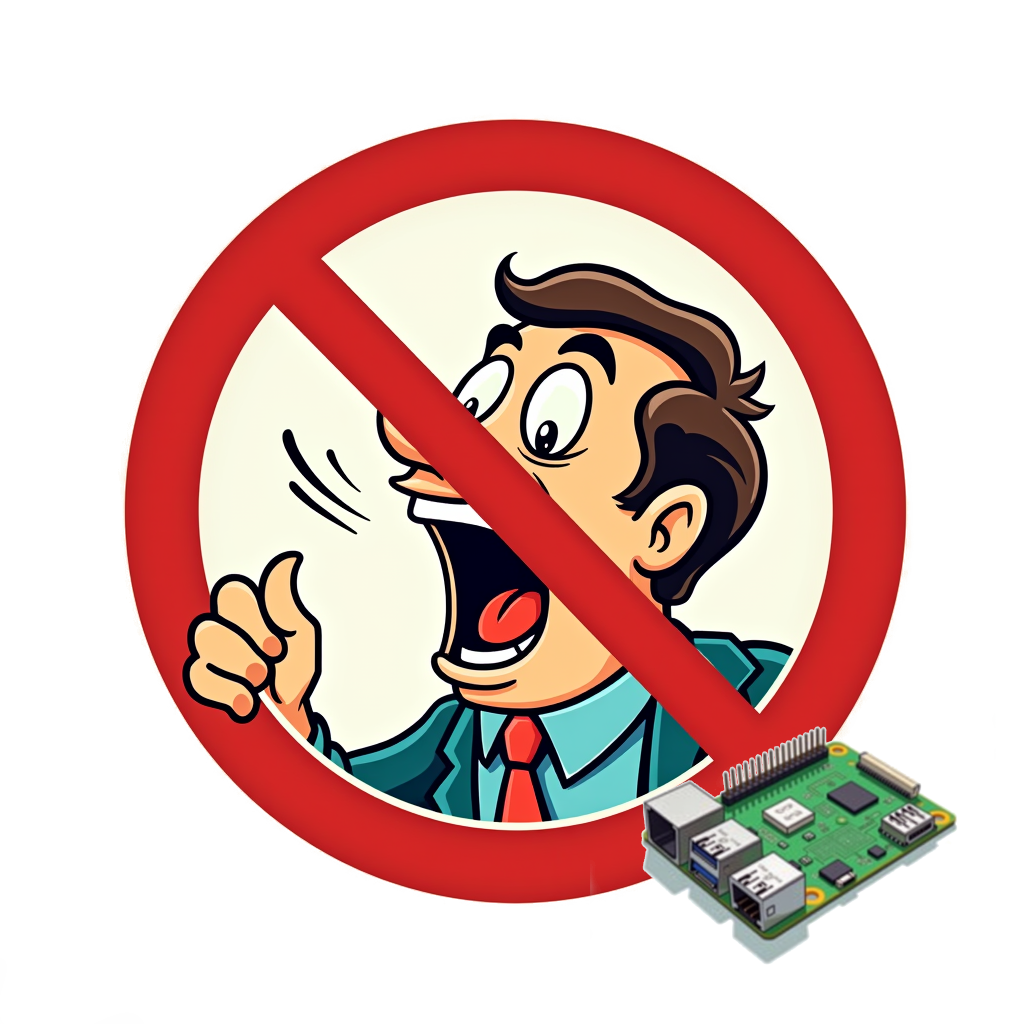
\includegraphics[scale=0.13]{Logo.png}}
	\end{center}
\end{frame}

\section{L'hardware}
\begin{frame}{L'hardware}
	\begin{itemize}
		\item Al momento della realizzazione l'hardware del progetto si compone di un "\href{https://www.maikii.com/faq/cose-un-power-bank/}{\textcolor{blue}{powerbank}}" che alimenta un "\href{https://www.raspberrypi.com/products/raspberry-pi-3-model-b-plus/}{\textcolor{blue}{Raspberry Pi 3B+}}" e un gruppo di altoparlanti di 5W di potenza. Gli altoparlanti sono collegati alla board tramite jack e alla stessa è poi connessa la "\href{https://it.wikipedia.org/wiki/PlayStation_Eye}{\textcolor{blue}{PlayStation Eye}}".
		\item Il "\href{https://www.raspberrypi.com/products/raspberry-pi-3-model-b-plus/}{\textcolor{blue}{Raspberry Pi 3B+}}" utilizza l'array di microfoni messo a disposizione dalla "\href{https://it.wikipedia.org/wiki/PlayStation_Eye}{\textcolor{blue}{PlayStation Eye}}" per monitorare il volume dei rumori presente nell'ambiente dove è posizionato il dispositivo e qualora i decibel rilevati dovessero superare la soglia, attraverso gli altoparlanti viene emesso un effetto eco.
	\end{itemize}
	\begin{center}
		\zoombox{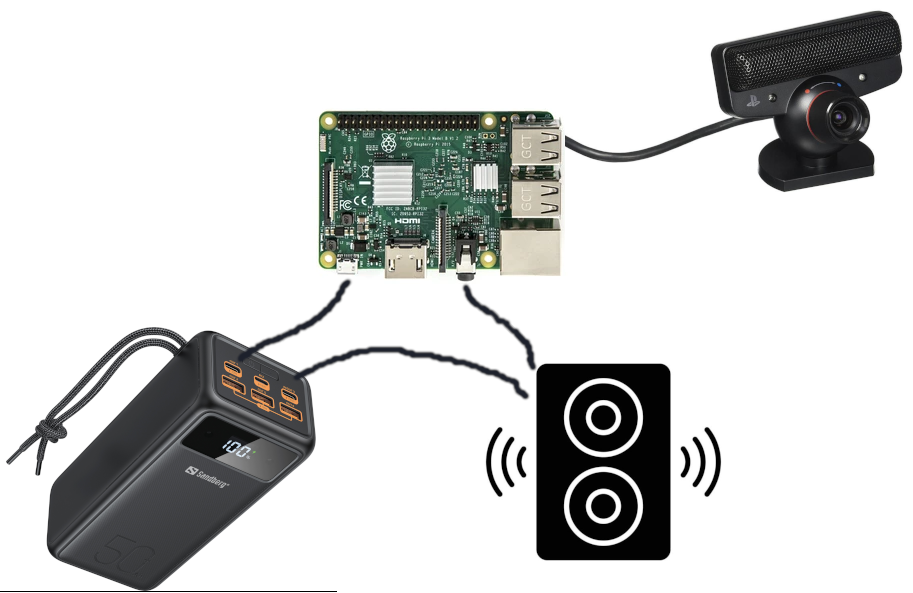
\includegraphics[scale=0.55]{schema.png}}
	\end{center}
\end{frame}

\section{Il software}
\begin{frame}{Il software}
	\begin{itemize}
		\item Il software principale è sviluppato in "\href{https://www.python.org/}{\textcolor{blue}{Python}}", il quale svolge la funzione di monitorare il volume dei rumori presente nelle stanza e di attivare l'eco qualora sia necessario, nel mentre che si registra il timestamp dell'evento e lo si manda a "\href{https://thingspeak.mathworks.com/}{\textcolor{blue}{ThingSpeak}}", oltre che viene aggiornato un file csv per la copia locale degli eventi.
		\item Utilizzando una combo di "\href{https://www.python.org/}{\textcolor{blue}{Python}}", "\href{https://it.wikipedia.org/wiki/JavaScript}{\textcolor{blue}{JavaScript}}" e il componente "\href{https://nginx.org/}{\textcolor{blue}{nginx}}" si espone all'indirizzo ip locale del dispositivo una pagina di controllo protetta da password.
	\end{itemize}
	\begin{center}
		\zoombox{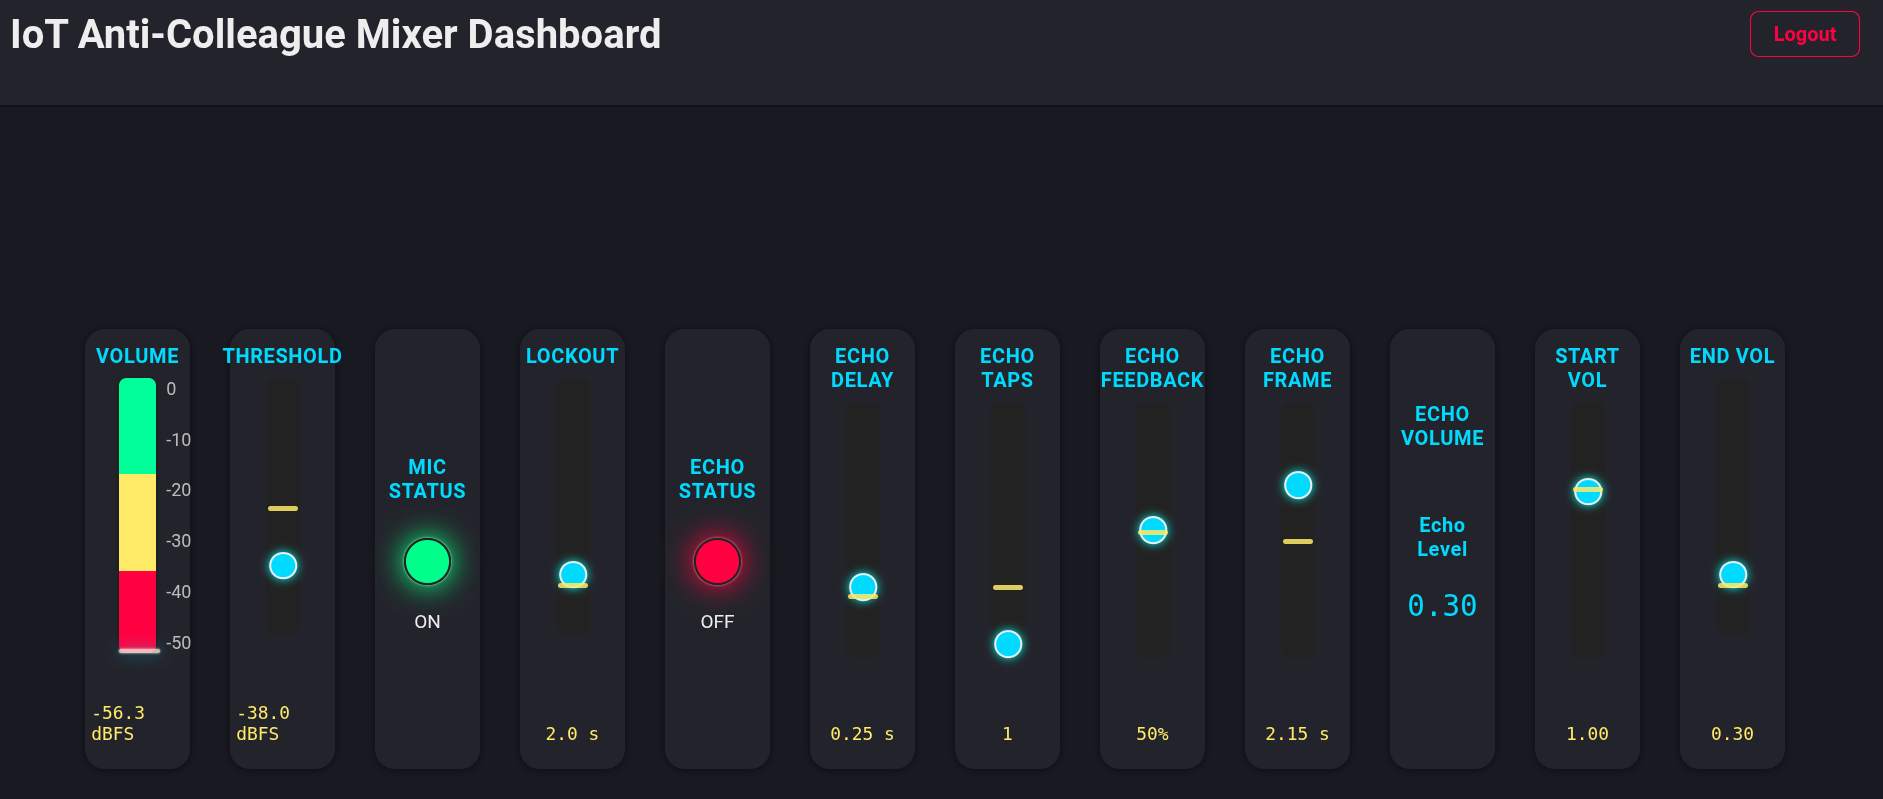
\includegraphics[scale=0.18]{mixer.png}}
	\end{center}
\end{frame}

\section{Sperimentazione sul campo}
\begin{frame}{Sperimentazione sul campo}
	\begin{tabularx}{\linewidth}{XX}
		{
			\centering
			\vspace*{-50mm}
			\begin{itemize}
				\item Il dispositivo è stato installato per due settimane all'interno dell'ambiente di lavoro prima citato e sono stati raccolti i relativi dati sul rumore. 
			\end{itemize}

		}&{
			\centering
			\zoombox{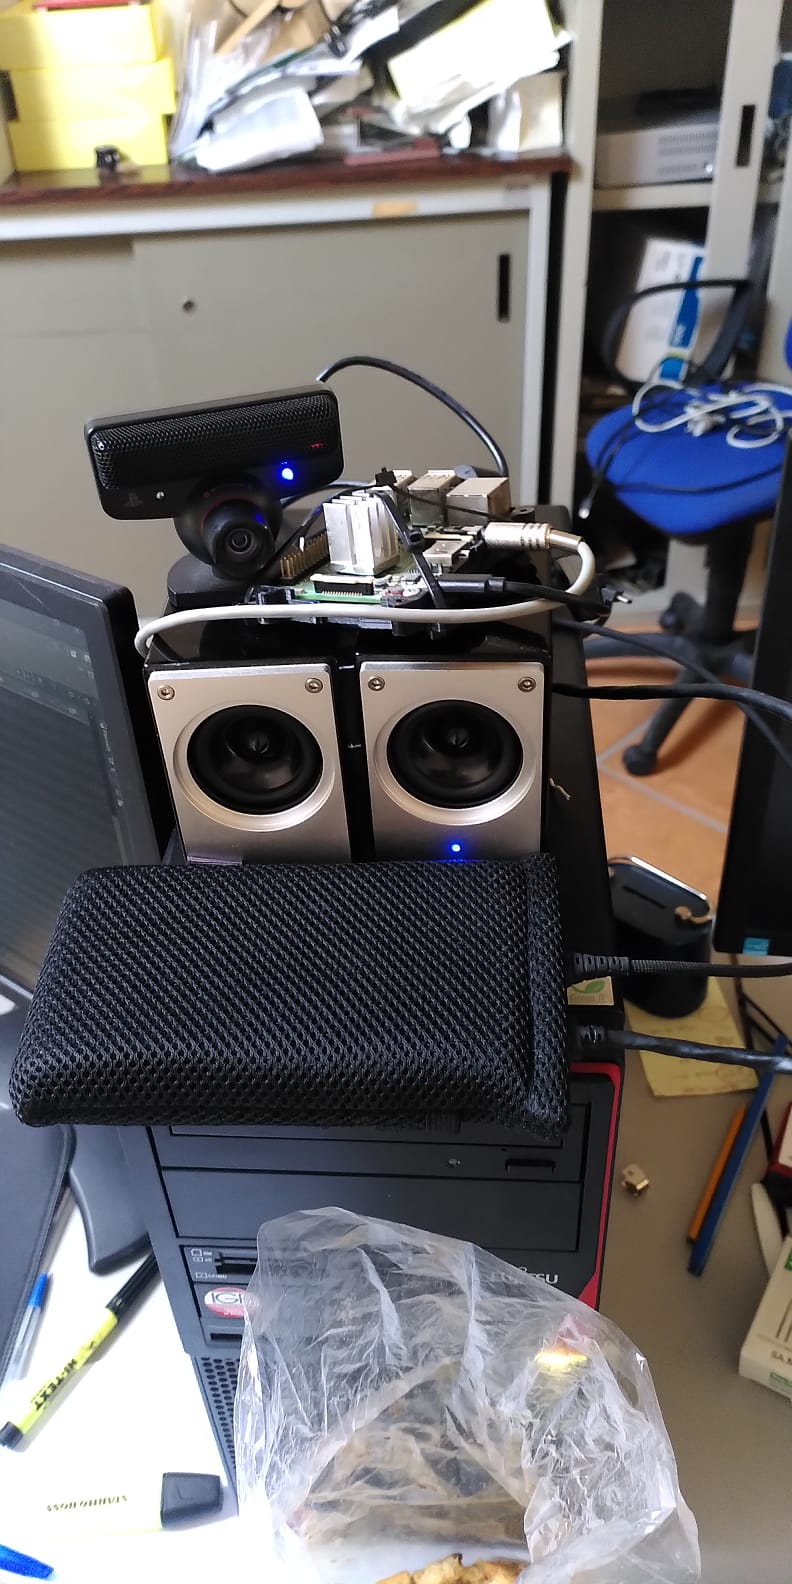
\includegraphics[scale=0.125]{work.jpeg}}
			
		}
	\end{tabularx}
\end{frame}

\section{Analisi dei dati}
\begin{frame}{Analisi dei dati}
	\begin{itemize}
		\item la raccolta dei dati mette in evidenza che durante il periodo di due settimane nel quale il dispositivo è stato in funzione, il rumore provocato dai colleghi poco rispettosi si è sensibilmente ridotto
	\end{itemize}
\vspace*{2mm}
	\begin{tabularx}{\linewidth}{XX}
		{
			\centering
			\zoombox{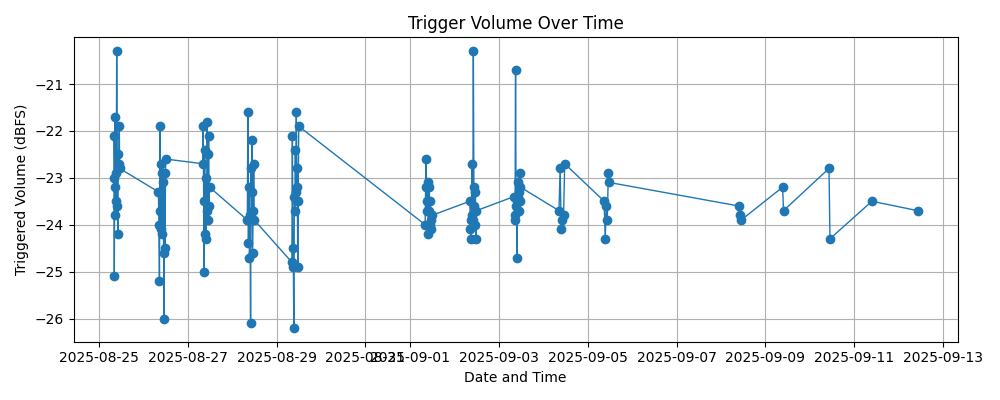
\includegraphics[scale=0.3]{trigger_volume_vs_time.png}}
			
			
		}&{
			\centering
			\zoombox{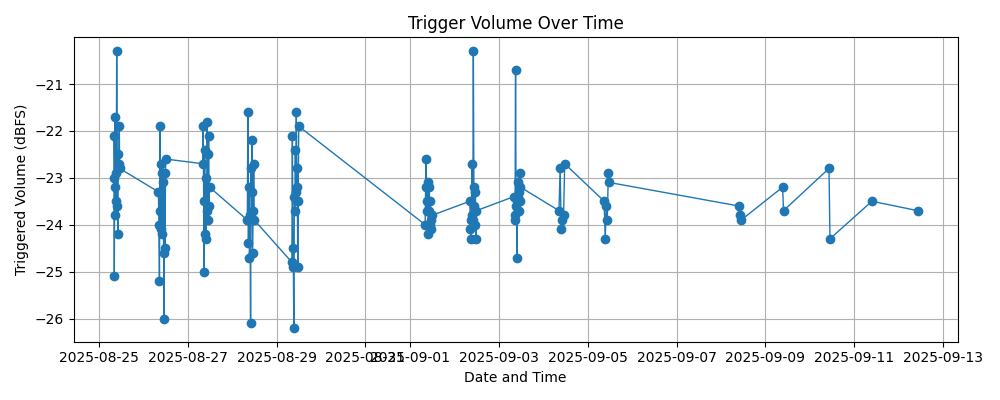
\includegraphics[scale=0.3]{trigger_volume_vs_time.png}}
			
		}
	\end{tabularx}
	
\end{frame}

\section{Valutazioni}
\begin{frame}{Valutazioni}
	\begin{itemize}
		\item Il sistema ha dimostrato la sua efficacia, sensibilizzando i colleghi a tenere toni di voce più consoni rispetto all'ambiente dove si trovano. 
		\item Su otto colleghi, solo un collega ha manifestato una certa avversione nei confronti del sistema, definendolo come troppo invasivo.
		\item In definitiva il dispositivo lo si può considerare come un sistema valido per mitigare in maniera efficacie il problema del rumore eccessivo negli ambienti di lavoro condivisi
	\end{itemize}
\end{frame}

\section{Conclusioni}
\begin{frame}{Conclusioni}
	\begin{itemize}
		\item l'esperimento condotto ha dimostrato la validità del dispositivo a mitigare i problemi descritti
		\item Tuttavia una soluzione di questo tipo non può essere adottata in modo continuativo e permanente, siccome la presenza costante dell'eco sonoro può far sorgere il senso dell'oppressione da parte delle persone che utilizzano l'ambiente monitorato.
		\item In conclusione si prevede di utilizzare il dispositivo con gli altoparlanti disattivati in modo da tenere attivo il controllo sui volumi, e di attivare quest'ultimi solo in caso di necessità e dopo aver condiviso l'intenzione con i presenti.
	\end{itemize}
\end{frame}
	
\end{document}